%08.02.2023 Аня

\subsection{Основная теорема арифметики}

\begin{reminder}
    Пусть $F$ -- поле. Многочлен $A$ ненулевой степени называется неприводимым над полем $F$, 
    если из $A = B \cdot C$, где $B, C \in F[x]$ следует, что $\deg B = 0$ или $\deg C = 0$.
\end{reminder}

\begin{proposition}
    Пусть $P$ -- неприводимый над $F$ и $P \, \vert \, (B \cdot C)$. Тогда $P \vert B$ или $P \vert C$.
\end{proposition}

\begin{proof}
    Покажем от противного: пусть $B$ и $C$ не кратны $P$. Тогда $\gd(B, P) = P$ или $\gd(B, P) = 1$.
    Первый вариант исключен по предположению, а значит $\gd(B, P) = 1$. Аналогично $\gd(C, P) = 1$.
    Тогда по теореме \ref{th1.4}: 
    \begin{gather*}
        \exists u_1, v_1 \in F[x]: u_1B + v_1P = 1,\\
        \exists u_2, v_2 \in F[x]: u_2C + v_2P = 1.
    \end{gather*}
    Перемножим левые части равенств: 
    $$u_1v_2BC + (u_1Bv_2 + u_2Cv_1 + v_1v_2P)P = 1$$
    Оба слагаемых в левой части равенства кратны $P$ -- противоречие.
\end{proof}

\begin{theorem} [основная теорема арифметики для многочлена]
    Пусть $F$ -- поле, $A \in F[x], A \neq 0$. Тогда верны следующие утверждения:
    \begin{enumerate}
        \item Существует разложение $A$ на неприводимые: $$A = \alpha P_1P_2 \dots P_n,$$ 
        где $\alpha \in F^*$, $P_i$ неприводимый над $F$ многочлен.
        \item Пусть A представляется в виде неприводимых многочленов двумя различными способами: 
        $$A = \alpha \cdot P_1P_2 \dots P_n = \beta \cdot Q_1Q_2 \dots Q_m,$$ 
        где $\beta\in F^*$, $Q_j$ -- неприводимый над $F$ многочлен. 

        Тогда $n = m$ и существует перестановка $\sigma\in S_n$ такая, что многочлены ассоциированы: 
        \begin{gather*}
            P_i \thicksim Q_j \, (1 \leq i \leq n), \text{ где } j = \sigma(i).
        \end{gather*}
    \end{enumerate}
\end{theorem}

\begin{proof}~
    \begin{enumerate}
        \item Докажем существование разложения на неприводимые множители индукцией по $\deg A$:
        \begin{enumerate}
            \item Если $\deg A = 0$, то $A = \alpha$, $\alpha \in F^*$. 
            \item Пусть $A$ неприводим над $F$, $\deg A \geq 1$. Будем считать, что в таком случае 
            разложение получено: $A = P$.

            Пусть теперь $A$ приводим над $F$, тогда его можно представить в виде $A = B \cdot C$, 
            $B, C \in F[x]$, $\deg B < \deg A$, $\deg C < \deg A$. Тогда  к $B$ и $C$ применимо 
            предположение индукции и, перемножая их, получим разложение для $A$.
        \end{enumerate}
        \item Пусть существуют два разложения многочлена $A$ на неприводимые:
        \begin{gather*}
            A = \alpha \cdot P_1P_2 \dots P_n = \beta \cdot Q_1Q_2...Q_m.
        \end{gather*}
        Покажем по индукции по $n$:
        \begin{enumerate}
            \item В случае $n=1$ из неприводимости $P_1$ следует, что $m$ так же равно единице.
            Таким образом, $A = \alpha \cdot P_1 = \beta \cdot Q_1$, а значит многочлены $P_1$ и $Q_1$ 
            ассоциированы. 
            \item Пусть теперь $n > 1$, тогда многочлен $P_n$ делит произведение $Q_1Q_2 \dots Q_m$.
            
            Тогда существует такое $j \in \{ 1, \dots, m\}$, что $P_n \vert Q_j$. 
            Из неприводимости многочленов $P_n$ и $Q_j$ существует такая $\gamma \in F^*$, что $Q_j = \gamma P_n$.
            Теперь можно подставить выражение для $Q_j$ в представление для $A$ справа:
            \begin{gather*}
                A = \alpha \cdot P_1P_2 \dots P_n = \beta \cdot Q_1Q_2 \dots Q_{j-1} \cdot \gamma 
                P_n \cdot Q_{j+1} \dots Q_m.
            \end{gather*} 
            
            Согласно утверждению \ref{pr1.3} 
            кольцо многочленов является областью целостности, а значит по утверждению \ref{pr1.2} 
            можно выполнить сокращение многочлена $P_n$ в обеих частях равенства. 
            
            По предположению индукции число множителей слева и справа после сокращения совпадает и 
            существует биекция $\sigma: \{ 1, \dots , n - 1\} \longrightarrow \{ 1, \dots , j - 1, j + 1, \dots , n \}$, 
            такая что $P_i \thicksim Q_{\sigma(i)}$. Доопределим биекцию: 
            $\sigma(n) = j$. Теперь $\sigma$ удовлетворяет всем условиям, 
            поэтому доказано для $n$.
        \end{enumerate}
    \end{enumerate}
\end{proof}

\begin{corollary}
    Пусть $A$ представим в виде $A = \alpha P_1^{k_1}P_2^{k_2} \dots P_s^{k_s}$ -- попарно не 
    ассоциированные неприводимые множители. Тогда утверждается, что всякий делитель $D\mid A$ 
    имеет вид: $$D = \beta P_1^{m_1}P_2^{m_2} \dots P_s^{m_s}, \text{ где } 0 \leq m_i \leq k_i.$$
\end{corollary}

\begin{proof}
    Очевидно, что разложение $D$ не может содержать множителей, не содержащихся в $A$, так как тогда $A$ будет иметь
    ещё одно разложение на неприводимые множители.
    Пусть $A$ представляется в виде $A = D \cdot Q$, где
    $Q = \alpha_1 P_1^{l_1}P_2^{l_2} \dots P_s^{l_s}$ и
    $D = \beta P_1^{m_1} \dots P_s^{m_s}$. Тогда $k_i = m_i + l_i$ и поэтому $0 \leq m_i \leq k_i$.
\end{proof}

\subsubsection{Кратные корни многочленов}

Пусть $f \in F[x]$, $c$ -- корень $f$. По теореме \ref{th1.2} Безу $(x-c) \vert f(x)$:
\begin{gather*}
    f(x) = q_1(x)(x - c).
\end{gather*}

При этом многочлен $q_1(x)$ так же может быть кратен $(x-c)$, а значит для некоторых $f(x)$ может 
существовать цепочка равенств:
\begin{gather*}
    f(x) = q_1(x)(x - c) = q_2(x)(x-c)^2 = \, \dots
\end{gather*}

\begin{definition}
    Корень многочлена $f(x)$ называется корнем кратности $k$ если $f$ кратно $(x-c)^k$, но не кратно $(x-c)^{k+1}$.
\end{definition}

\begin{note}
    $c$ -- корень кратности $k$ $\lra f(x) = q_k(x) (x-c)^k$, $q_k(c) \neq 0$.
\end{note}

\begin{proposition}
    \label{pr1.7}
    Пусть $f$ - многочлен из $F[x]$. Тогда сумма кратностей всех корней многочлена $f$ не превосходит $n = \deg(f)$
\end{proposition}

\begin{proof}
    Пусть $c_1$, $c_2$, $\dots c_s$ - корни многочлена, $k_1$ ,$k_2$, $\dots ,k_s$ -- соответствующие им 
    кратности: 
    \begin{gather*}
        f(x) \, \vdots \, (x - c_1)^{k_1}, \\
        \dots \\
        f(x) \, \vdots \, (x - c_s)^{k_s}.
    \end{gather*}
    При этом многочлены $(x-c_i)$ и $(x-c_j)$ неприводимы и неассоциированы для всех различных $i$ и $j$. 
    Это очевидно, так как они имеют первую степень, а значит разложиться могли бы только в произведение констант. 
    Поэтому многочлен $f(x)$ кратен так же произведению $(x-c_i)$ в соответствующих степенях:
    \begin{gather*}
        f(x) \, \vdots \, (x-c_1)^{k_1} \cdot \, \dots \, \cdot (x-c_s)^{k_s}.
    \end{gather*}
    Таким образом, сумма степеней не превосходит степень $f(x)$.
\end{proof}

\begin{note}
    Рассмотрим кольцо $\Z_6[x]$ и многочлен $f(x) = x^2 + x$ над ним. Он имеет четыре корня - $0$, $2$, $3$, $5$, 
    а значит сумма кратностей корней гарантированно превосходит степень многочлена. 
    Является ли это противоречием к утверждению \ref{pr1.7}? Нет, потому что $\Z_6[x]$ не является полем.
    Заметим, что здесь ещё и разложение на неприводимые не является единственным: 
    $$x^2 + x = x(x+1) = (x+3)(x+4).$$
    И снова это происходит потому что основная теорема арифметики доказана в предположении многочлена над полем.
\end{note}

\subsection{Основная теорема алгебры}

\begin{definition}
    Если F -- поле, такое что в кольце $F[x]$ всякий многочлен имеет хотя бы один корень из $F$, то 
    $F$ алгебраически замкнуто.
\end{definition}

\begin{theorem}[Основная теорема алгебры]~
    \label{ota}

    Всякий многочлен положительной степени из кольца $\Cm[x]$ имеет хотя бы один корень, в общем случае комплексный.
    Альтернативная формулировка: поле комплексных чисел алгебраически замкнуто.
\end{theorem}

\begin{definition}
    Будем говорить, что для комплексной последовательности $z_n$ существует предел 
    $\displaystyle\lim_{n\to \infty} {z_n} = z$, 
    если существует предел действительной последовательности $\displaystyle\lim_{n\to \infty} {|z_n - z|} = 0$.
\end{definition}

\begin{agreement}
    Далее будем использовать обозначения: $z_n = x_n + i y_n$, $z = x + i y$.
\end{agreement}

\begin{lemma}
    \label{lemma1}
    $\exists \displaystyle\lim_{n\to \infty} {z_n} = z \lra$ $\exists \displaystyle\lim_{n\to \infty} {x_n} = x, \exists \displaystyle\lim_{n\to \infty} {y_n} = y$.
\end{lemma}

\begin{idea}
    Теорема Пифагора.
\end{idea}

\begin{lemma}
    \label{lemma2}
    Если существует предел $\displaystyle\lim_{n\to \infty} {z_n} = z$, то существует и предел $\displaystyle\lim_{n\to \infty} {|z_n|} = |z|$.
\end{lemma}

\begin{idea}
    Использовать неравенство треугольника.
\end{idea}

\begin{lemma}
    \label{lemma3}
    Если для комплексных последовательностей $z_n$ и $w_n$ существуют пределы \\
    $\displaystyle\lim_{n\to \infty} {z_n} = z$ и $\displaystyle\lim_{n\to \infty} {w_n} = w$, 
    то существуют и пределы $\displaystyle\lim_{n\to \infty} {z_n + w_n} = z + w$ и 
    $\displaystyle\lim_{n\to \infty} {z_n \cdot w_n} = z \cdot w$.
\end{lemma}

\begin{idea}
    Воспользоваться аналогичными свойствами пределов действительных последовательностей из курса 
    математического анализа первого семестра.
\end{idea}

\begin{note}
    Фактически лемма равносильна тому, что многочлен является непрерывной функцией над полем $\Cm$.
\end{note}

\begin{definition}
    Будем говорить, что последовательность $z_n$ сходится к бесконечности, если для действительной 
    последовательности $|z_n|$ существует предел $\displaystyle\lim_{n\to \infty} {|z_n|} = +\infty$.
\end{definition}

\begin{lemma}
    \label{lemma4}
    Пусть $\{ z_n \}$ -- произвольная последовательность поля $\Cm$. Тогда из нее можно извлечь подпоследовательность,
    сходящуюся к конечному числу $z_0$ или к бесконечности.
\end{lemma}

\begin{proof}~
    \begin{enumerate}
        \item Пусть существует константа $C > 0$, такая что для всех $n$ верно $|z_n| \leq C$. 
        
        Тогда, так как верно $|x_n| \leq |z_n|$, последовательность $\{ x_n \}$ ограничена,
        а значит, по теореме Больцано-Вейерштрасса из неё можно извлечь сходящуюся подпоследовательность $x_{n_k}$.
        
        Рассмотрим теперь последовательность $\{y_{n_k}\}$, являющуюся подпоследовательностью $\{y_n\}$ с индексами, 
        соответствующими сходящейся подпоследовательности $\{x_n\}$.
        Аналогично для этой последовательности верно $|y_{n_k}| \leq |z_{n_k}|$ для всех $n_k$, 
        а значит последовательность ограничена, и теореме Больцано-Вейерштрасса из 
        неё можно извлечь сходящуюся подпоследовательность $\{y_{n_{k_s}}\}$. 
        
        Для упрощения записи обозначим $i = n_{k_s}$.
        Тогда последовательности $\{x_i\}$ и $\{y_i\}$ сходятся, а значит сходится и 
        соответствующая последовательность $\{ z_n \}$ (по лемме \ref{lemma1}).
        
        \item 
        Пусть теперь $\{ |z_n| \}$ не ограничена. Тогда из нее можно извлечь подпоследовательность с 
        монотонно возрастающим модулем (сходящуюся к бесконечности) следующим образом:
        
        Из неограниченности получим $\forall N \; \exists k: |z_k| > N$. Построим тогда подпоследовательность $z_i = z_{n_k}$,
        каждый раз выбирая $n_k$ так чтобы $z_{n_k}$ было больше $i$ и $n_k > n_{k-1}$. Таким образом $z_{n_k}$ стремится к бесконечности.
    \end{enumerate}
\end{proof}

\begin{lemma}
    \label{lemma5}
    Пусть $f \in \Cm[x]$ и $\deg f = m \geq 1$. Тогда если $z_n$ сходится к бесконечности то $f(z_n)$ сходится к бесконечности.
\end{lemma}

\begin{proof}
    Представим многочлен $f(x)$ в следующем виде:
    $$f(z) = a_0 z^m + a_1 z^{m-1} \dots + a_{m-1} z + a_m = z^m (a_0 + \frac{a_1}{z} + \dots + \frac{a_m}{z^m}), \; a_0 \neq 0.$$
    Подставим последовательность $z_n$. Тогда модуль $|z_n|^m$ сходится к бесконечности, а значение 
    в скобках сходится к $a_0$, так как мы положили его ненулевым. Отсюда $|f(z_n)|$ сходится 
    к бесконечности, и значит, $f(z_n)$ тоже сходится к бесконечности.
\end{proof}

\begin{reminder}
    $e^{i\phi} = \cos(\phi) + i\sin(\phi)$.
\end{reminder}

\begin{lemma}[Д'Аламбера]
    \label{lemma6}
    Пусть $f(x)$ -- многочлен положительной степени из кольца $\Cm[z]$, имеющий в $z_0$ ненулевое 
    значение: $f(z_0) \neq 0$. Тогда для любой $\epsilon$-окрестности $U_{\varepsilon}(z_0)$ найдется 
    $z \in U_{\varepsilon}(z_0)$, такое что $|f(z)| < |f(z_0)|$.
\end{lemma}

\begin{proof}~
    \begin{enumerate}
        \item Зафиксируем $\varepsilon > 0$. Разделим $f(z)$ на $z - z_0$ с остатком. Мы знаем, 
        что остаток имеет смысл значения многочлена в точке $z_0$. Таким образом,
        $f(z) = q_1(z) (z-z_0) + r_0$, где $r_0 = f(z_0)$. 
        \item Разделим теперь многочлен $q_1$ на $z - z_0$ и подставим полученное выражение
        в полученное выше разложение для $f$. Получаем $f = q_2(z)(z-z_0)^2 + r_1(z-z_0) + r_0$, где $r_1 = q_1(z_0)$. 
        \item Продолжим делить остатки на $z-z_0$ и получим следующее выражение для $f(x)$:
        \begin{gather*}
            f(z) = f(z_0) + \frac{f'(z)}{1!}(z - z_0) + \frac{f''(z_0)}{2!}(z - z_0)^2 + \dots.
        \end{gather*}
        В выражении выше $r_0 = f(z_0)$, $r_1 = f'(z_0)$, $\dots$, $r_k = \frac {f^{(k)}(z_0)}{k!}$. 
        Такое разложение напоминает разложение в ряд Тейлора.
        \item 
        Обозначим главную часть за $\alpha (z - z_0)^p, \alpha \neq 0, p \in \N$. Получим представление 
        $f(z)$ в виде:
        \begin{gather*}
            f(z) = f(z_0) + \alpha (z-z_0)^p + o(z-z_0)^p = f(z_0) + (z - z_0)^p \left( \alpha + 
            \frac{o(z-z_0)^p}{(z-z_0)^p} \right),
        \end{gather*}
        при этом $o(z - z_0)^p $ кратно $(z - z_0)^p$. Так как последнее частное стремится 
        к 0 при $z$, стремящимся к $z_0$, верно:
        \begin{gather*}
            \exists \varepsilon_1 < \varepsilon: \, \forall z \in U_{\varepsilon_1}(z_0) \hookrightarrow 
            \left| \frac {o(z-z_0)^p}{(z-z_0)^p} \right| < \frac {|\alpha |}{2}. 
        \end{gather*}
        Таким образом:
        \begin{gather*}
            \arg(\alpha) - \frac {\pi}{6} \leq \arg(\alpha + \frac {o(z - z_0)^p}{(z - z_0)^p}) \leq 
            \arg(\alpha) + \frac {\pi}{6}; \; \alpha \in [\alpha_0; \alpha_0 + \frac {\pi}{3}]
        \end{gather*}
        Тогда если записать $z$ как $z = z_0 + r \cdot e^{i\phi}$, где $r = |z|$, $e^{i\phi} = \cos(\phi) + i\sin(\phi)$, то справедливо:
        $$\arg \left( e^{\pi\phi} \left( \alpha + \frac {o(z-z_0)^p}{(z-z_0)^p}\right) \right) = 
        \pi \phi + \alpha_0 + \beta \cdot \frac{\pi}{3}; 0 \leq \beta \leq 1$$
        Так как $\phi$ -- любое вещественное число, то теорема доказана.
    \end{enumerate}

    \begin{center}
        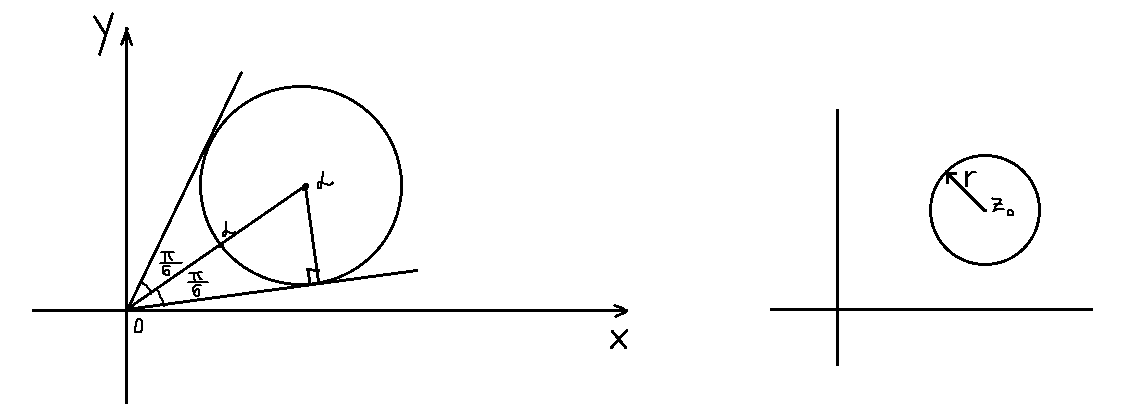
\includegraphics[width=1\textwidth]{images/lec2_1.png}
    \end{center}
\end{proof}

\begin{note}
    Идея леммы заключается в том, чтобы приблизить значение $z$ к $z_0$, то есть найти значение, 
    при котором $|f(z)| < |f(z_0)|$, но при этом сколь угодно близкое к $z_0$. 
\end{note}

\begin{reminder}
    Основная теорема алгебры утверждает, что любой многочлен в поле комплексных чисел имеет хотя бы один корень.
\end{reminder}

\begin{proof}
    Пусть $f(x)$ -- многочлены положительной степени. Пусть $A = \inf |f(z)|$, $z \in \Cm$. 
    Покажем, что инфимум достигается, то есть что существует такое комплексное число $z_n \in \Cm$, 
    что $|f(z_n)| = A$:
    \begin{enumerate}
        \item 
        По определению инфимума существует последовательность ${z_n}$ такая, что $|f(z_n)|$ стремится к конечному $A$. 
        \item 
        По лемме \ref{lemma4} из неё можно извлечь подпоследовательность ${z_{n_k}}$ такую, что она 
        сходится к $z_0$ или к бесконечности. 
        \item 
        По лемме \ref{lemma5} второй случай не реализуется, так как иначе $|f(z_{n_k})|$ также 
        сходится к бесконечности. 
        \item 
        Тогда для подпоследовательности существует конечный предел $\displaystyle\lim_{k\to \infty} 
        {z_{n_k}} = z_0 \in \Cm$, откуда существует и предел $\displaystyle\lim_{k\to \infty} 
        {f(z_{n_k})} = f(z_0)$, а значит, по лемме \ref{lemma2}, существует предел модуля такой функции, равный
        $\displaystyle\lim_{k\to \infty} {|f(z_{n_k})|} = |f(z_0)| = A$. 
        \item 
        Если оказалось так, что $A \neq 0$, то по лемме \ref{lemma6} найдется $z \in U_{\epsilon}(z)$ такой что:
        $$|f(x)| < |f(z_0)| = A = inf(|f(z)|),$$ что противоречит определению инфимума. Таким образом $A = 0$
        и инфимум достигается, а значит $f(z)$ имеет хотя бы один корень.
    \end{enumerate} 
\end{proof}

\subsubsection{Следствия из основной теоремы алгебры}

\begin{corollary}
    Всякий многочлен $f$ положительной степени из кольца $\Cm[z]$ можно разложить в произведение 
    линейных многочленов из $\Cm[z]$.
\end{corollary}

\begin{proof}
    По основной теореме алгебры у $f$ существует хотя бы один корень $c_1$. Тогда справедливо представление: 
    $$f(z) = q_1(z) (z - c_1) = q_2(z)(z - c_1)(z - c_2) \dots = \alpha (z - c_1)(z - c_2) \dots (z - c_n),$$ 
    где $\deg f = n$.
\end{proof}

\begin{corollary}
    Всякий многочлен $f$ степени $n$ из $\Cm[z]$ имеет ровно $n$ корней в $\Cm$, если каждый корень 
    учесть с его кратностью.
\end{corollary}

\begin{proof}
    $f(z) = \alpha(z-c_1)^{k_1}\dots(z - c_s)^{k_s}$, $n = k_1 + \dots + k_s$, где $k_i$ -- кратность корня $c_i$.
\end{proof}

\begin{corollary}
    Если $f \in \R[x]$ и $c \in \Cm \backslash \R$ -- корень $f$ кратности $k$, то $\overline{c}$ тоже корень $f$ той же кратности $k$.
\end{corollary}

\begin{proof}
    \begin{align*}
        f(x) & = a_0 x^n + \, \dots \, + a_{n-1} x + a_n, \\
        f(c) & = a_0 c^n + \, \dots \, + a_{n-1} c + a_n = 0, \\
        f(\overline{c}) & = a_0 \overline{c}^n + \, \dots \, + a_{n-1} \overline{c} + a_n = 0.
    \end{align*}
    Кратность $c$ как корня $f$ равна количеству нулевых остатков $r_0$, $r_1$, $\dots$, $r_n$
    Для доказательства кратности сопряженного применим сопряжение ко всей схеме Горнера.
\end{proof}

\begin{corollary}
    Всякий многочлен $f \in \R[x]$, $\deg(f) \geq 1$ раскладывается над $\R[x]$ в произведение многочленов
    1-ой и 2-ой степеней, причем квадратные многочлены имеют отрицательный дискриминант.
\end{corollary}

\begin{proof}
    Индукция по степени $f$:
    \begin{enumerate}
        \item Если $\deg f = 1$ или $\deg f = 2$, то истинность очевидна.
        \item Пусть теперь многочлен имеет степень, большую $2$. Пусть $c$ -- корень $f$, $c \in \R$, то есть
        справедливо представление $f(x) = q(x)(x-c)$. Тогда по предположению индукции можно разложить 
        $q(x)$ и получить разложение для $f(x)$. 

        Теперь пусть $c \in \Cm \backslash \R$. Тогда $f$ кратен $x - c$ и $x - \overline{c}$, 
        а значит, кратен их произведению: $$f(x) = q(x)(x^2 - 2 Re(c) \cdot x + |c|^2).$$
        Произведение корней, в свою очередь, является многочленом степени $2$ из кольца $\R[x]$, 
        имеющим отрицательный дискриминант. Остается только применить предположение индукции к 
        многочлену $q(x)$.
    \end{enumerate}
\end{proof}

\begin{corollary}
    Всякий многочлен из $\R[x]$ положительной нечетной степени имеет хотя бы один действительный корень.
\end{corollary}

\begin{proof}
    Действительно, если многочлен имеет комплексный корень, то сопряженное к нему число также является корнем.
    Тогда если отбросить все комплексные корни, то мы отбросим четное число корней, а значит, останется 
    хотя бы один действительный корень.
\end{proof}

\begin{corollary}[об описании неприводимых многочленов над полями $\R$, $\Cm$]~
    \begin{enumerate}
        \item Над полем комплексных чисел $\Cm$ неприводимыми являются многочлены первой степени и только они.
        \item Над полем действительных чисел $\R$ неприводимыми являются многочлены первой степени и многочлены второй степени с отрицательным дискриминантом.
    \end{enumerate}
\end{corollary}

\begin{proposition}
    Для любого натурального $n \in \N$ существует многочлен из $\Q[x]$ степени $n$, являющийся неприводимым над $\Q$.
\end{proposition}

\begin{example}
    $x^2 + 2$ -- неприводим, $x^3 + 2$ -- неприводим $\dots $ $x^n + 2$ -- неприводим. Для 
    доказательства нужно использовать достаточное условие Эйзенштейна.
\end{example}

\begin{remarkfrom}
Критерий Эйзенштейна приведен, например, в лекциях Вадима Владимировича 2021го года:

Пусть многочлен $f(x)$ представим в следующем виде: 
$$f(x) = a_0x^n + a_1x^{n - 1} + \dots + a_{n - 1}x + a_n, \; a_i \in \Z.$$ 
Если существует такое простое число $p$, что $p \vert a_0$ и $p \vert a_i \; \forall i > 0, p \vert a_n$, но $a_n$ не делится на $p^2$, то $f(x)$ неприводим над $\Q$. 
\end{remarkfrom}

\begin{idea}
    Доказывается от противного. Предположим, что многочлен приводим, тогда существует его разложение 
    на произведение двух многочленов. После этого попробуем получить коэффициенты в явном виде - должно получиться.)
\end{idea}
